\documentclass[UTF8]{article}
\usepackage{ctex}
\usepackage{geometry}
\geometry{a4paper, scale=0.8}
\usepackage{graphicx}
\usepackage{subfigure}
\usepackage{float}
\usepackage{fontspec}
\newfontfamily\jetbrains{JetBrains Mono}
\usepackage{listings}
\usepackage{color}
\lstset{
    breaklines,                                 % 自动将长的代码行换行排版
    extendedchars=false,                        % 解决代码跨页时,章节标题,页眉等汉字不显示的问题
    backgroundcolor=\color[rgb]{0.96,0.96,0.96},% 背景颜色
    keywordstyle=\color{blue}\bfseries,         % 关键字颜色
    identifierstyle=\color{black},              % 普通标识符颜色
    commentstyle=\color[rgb]{0,0.6,0},          % 注释颜色
    stringstyle=\color[rgb]{0.58,0,0.82},       % 字符串颜色
    showstringspaces=false,                     % 不显示字符串内的空格
    numbers=left,                               % 显示行号
    numberstyle=\tiny\jetbrains,                    % 设置数字字体
    basicstyle=\small\jetbrains,                    % 设置基本字体
    captionpos=t,                               % title在上方(在bottom即为b)
    frame=single,                               % 设置代码框形式
    rulecolor=\color[rgb]{0.8,0.8,0.8},         % 设置代码框颜色
}
% \usepackage{bookmark}
\usepackage{enumitem}
\usepackage{hyperref}
\hypersetup{
    hypertex=true,
    colorlinks=true,
    linkcolor=black,
    anchorcolor=black,
    citecolor=black,
}


\title{Verilog实验\ lab3实验报告}
\author{PB19071405\ 王昊元}
\date{2022 年 05 月 01 日}

\begin{document}
    \maketitle

    \section{实验目的}
    \begin{enumerate}
        \item 权衡cache size增大带来的命中率提升收益和存储资源电路面积的开销
        \item 权衡选择合适的组相连度(相连度增大cache size也会增大,但是冲突miss会减低)
        \item 体会使用复杂电路实现复杂替换策略带来的收益和简单替换策略的优势(有时候简单策略比复杂策略效果不差很多甚至可能更好)
        \item 理解写回法的优劣
    \end{enumerate}
    \section{实验要求}
    \begin{enumerate}
        \item 理解提供的直接映射策略的cache,将它修改为N路组相连的cache,并通过cache读写测试。
        \item 使用编写的N路组相连cache正确运行提供的几个程序。
        \item 对不同cache策略和参数进行性能和资源的测试评估,编写实验报告。
    \end{enumerate}
    \section{实验环境}
    \begin{itemize}
        \item vlab
        \item Vivado 2016.3
    \end{itemize}
    \section{实验核心实现}
    \begin{enumerate}
        \item 在直接映射策略的cache上进行一些改动,例如改变{\jetbrains cache\_mem}、{\jetbrains cache\_tags}等的数组维数,
        修改命中规则(即改成对组内每一个line进行判断,并记录line在组内的索引),此外还需要修改状态机的状态跳转过程,这是由cache相关数组维数改变所引起的。
        \item 在基本的改动之后,需要实现N路组相连cache的换出策略,FIFO和LRU两种策略,我们通过维护一个{\jetbrains info}变量来实现。
        对于FIFO策略,{\jetbrains info}变量记录该line从进入cache到现在的时间,对于LRU则记录从上次被命中到现在的时间,
        而两种策略都取各自时间最久的来换出,这也是使用一个变量可以维护两种策略的原因。
        此时只需要在未命中的部分添加选择要换出的line索引即可(实现中命中line的索引和该处未命中要换出line的索引用同一变量维护)。
        此外,由于只有时间的绝对大小并没有实际作用,所以我们对于FIFO策略,只在换入换出时更新{\jetbrains info},
        因为命中时该组每个line对应的数值都加1,相对大小不变,不影响换出。下为该部分代码实现:\\
        \begin{lstlisting}[language=verilog]
// maintain info variable
always @ (posedge clk or posedge rst)
begin
    if(rst)
    begin
        for(integer i = 0; i < SET_SIZE; i++)
        begin
            for(integer j = 0; j < WAY_CNT; j++)
            begin
                info[i][j] <= 32'b0;
            end
        end
    end
    else
    begin
        if(mode == FIFO)
        begin
            // 考虑到在没有换入换出的情况下,所有info都+1不会改变它们的大小关系,故只在有换入换出时维护info
            if(cache_stat == SWAP_IN_OK)
            begin
                for(integer i = 0; i < WAY_CNT; i++)
                begin
                    if(i == mem_line_idx)
                    begin
                        info[set_addr][i] <= 32'b0;
                    end
                    else
                    begin
                        info[set_addr][i] <= info[set_addr][i] + 1;
                    end
                end
            end
        end
        else if(mode == LRU)
        begin
            if(signal && miss == 1'b0)  // if hit
            begin
                for(integer i = 0; i < WAY_CNT; i++)
                begin
                    if(i == line_idx)
                    begin
                        info[set_addr][i] <= 32'b0;
                    end
                    else
                    begin
                        info[set_addr][i] <= info[set_addr][i] + 1;
                    end
                end
            end
            else if(cache_stat == SWAP_IN_OK)  // if not hit, then swap, and only update info when swap finish.
            begin
                for(integer i = 0; i < WAY_CNT; i++)
                begin
                    if(i == mem_line_idx)
                    begin
                        info[set_addr][i] <= 32'b0;
                    end
                    else
                    begin
                        info[set_addr][i] <= info[set_addr][i] + 1;
                    end
                end
            end
        end
    end
end
        \end{lstlisting}
        \item 除此之外,需要对CPU的{\jetbrains Hazard}部分进行修改,在cache miss时,CPU stall。
    \end{enumerate}
    \section{实验结果及分析}
    \subsection{阶段一结果验证}
    \begin{figure}[H]
        \centering
        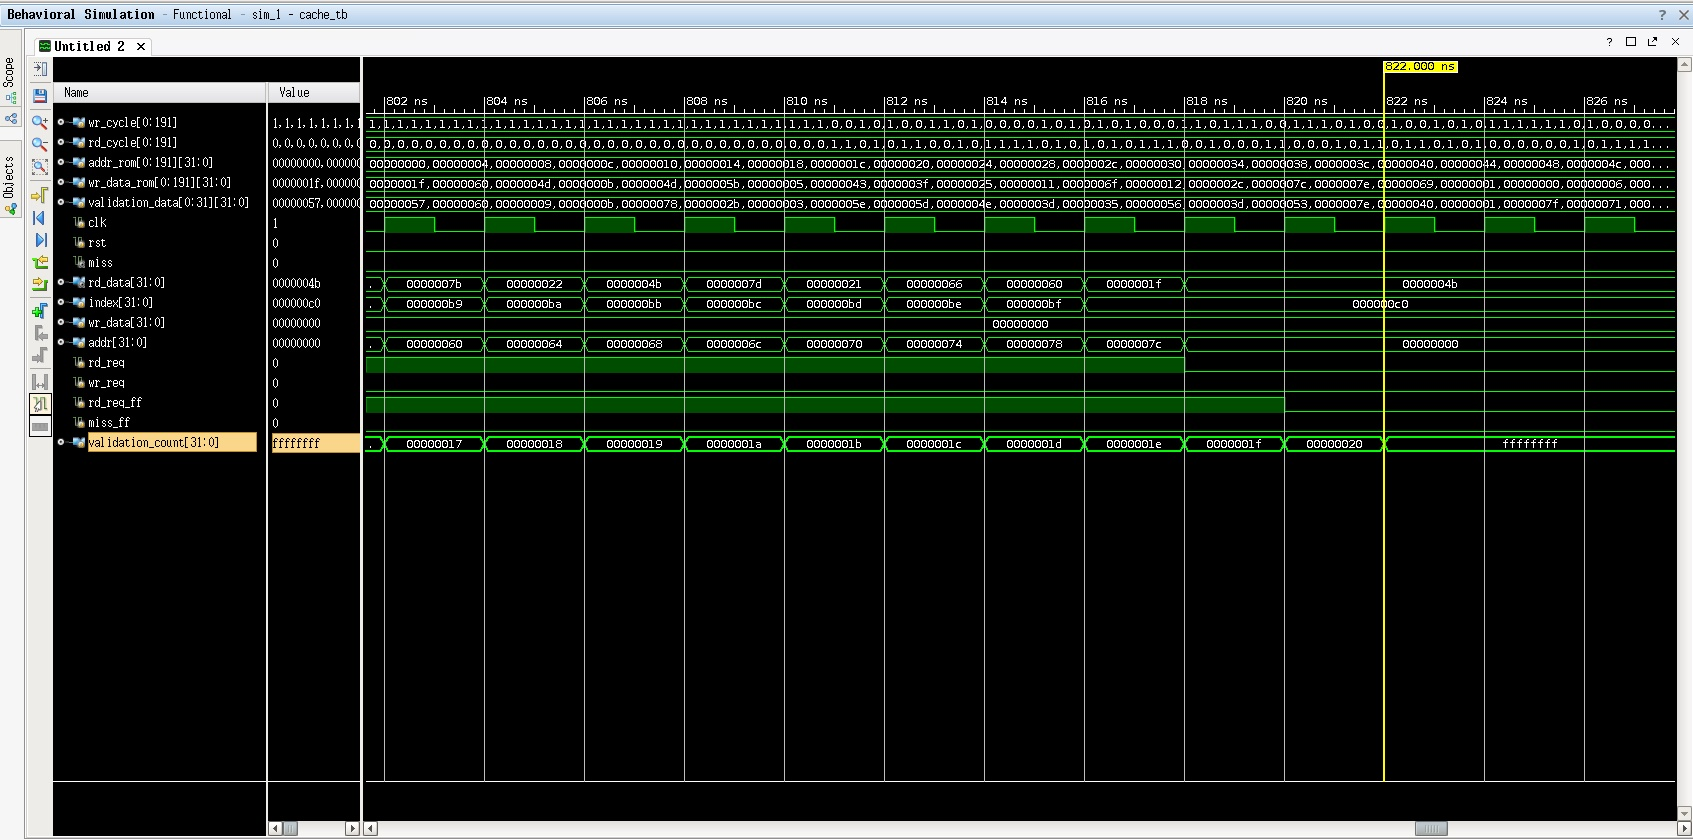
\includegraphics[width=0.8\textwidth]{./fig/stage1.jpg}
        \caption{阶段一结果截图}
        \label{stage1}
    \end{figure}
    从图\ref{stage1}可以看出,{\jetbrains validation\_count}不断增加,
    最后变为{\jetbrains ffffffff},通过了cache读写测试。
    \subsection{阶段二结果验证}
    因为个人没有windows系统,不方便生成太多不同规模的程序,
    故以下结果验证及分析阶段只使用规模为256的快排及规模为16的矩阵乘法进行。

    下面结果验证部分的cache参数为{\jetbrains LINE\_ADDR\_LEN\ =\ 3\ SET\_ADDR\_LEN\ =\ 3\ TAG\_ADDR\_LEN\ =\ 6\ WAY\_CNT\ =\ 4}。
    \begin{enumerate}[label=(\arabic*)]
        \item FIFO策略
        \begin{figure}[H]
            \centering
            \subfigure[快排]{
                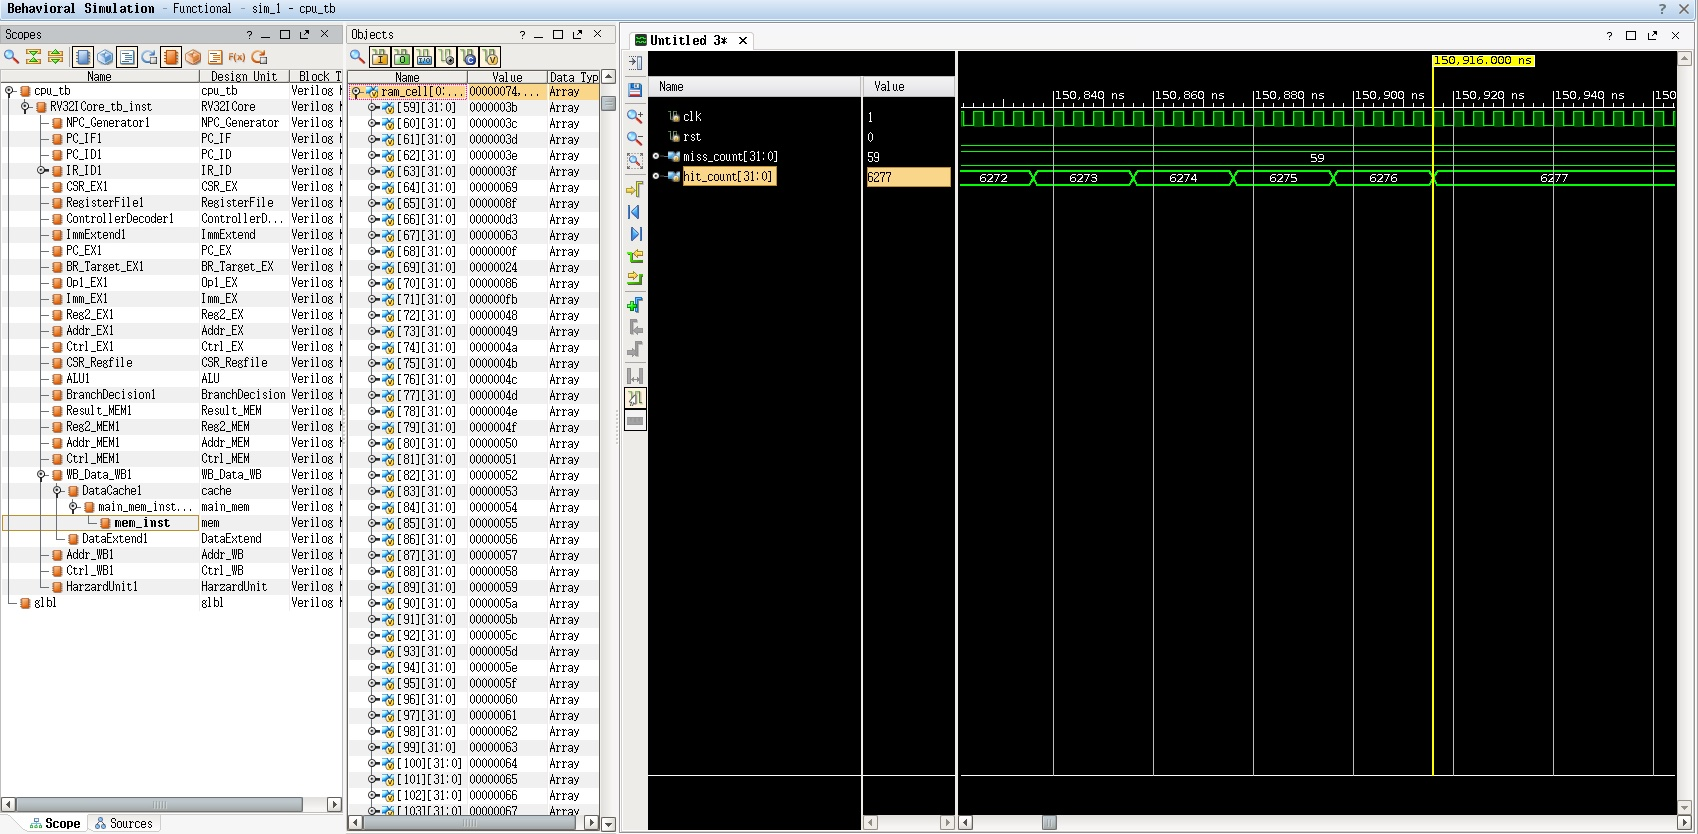
\includegraphics[width=0.4\textwidth]{./fig/stage2_fifo_qsort.jpg}
            }
            \subfigure[矩阵乘法]{
                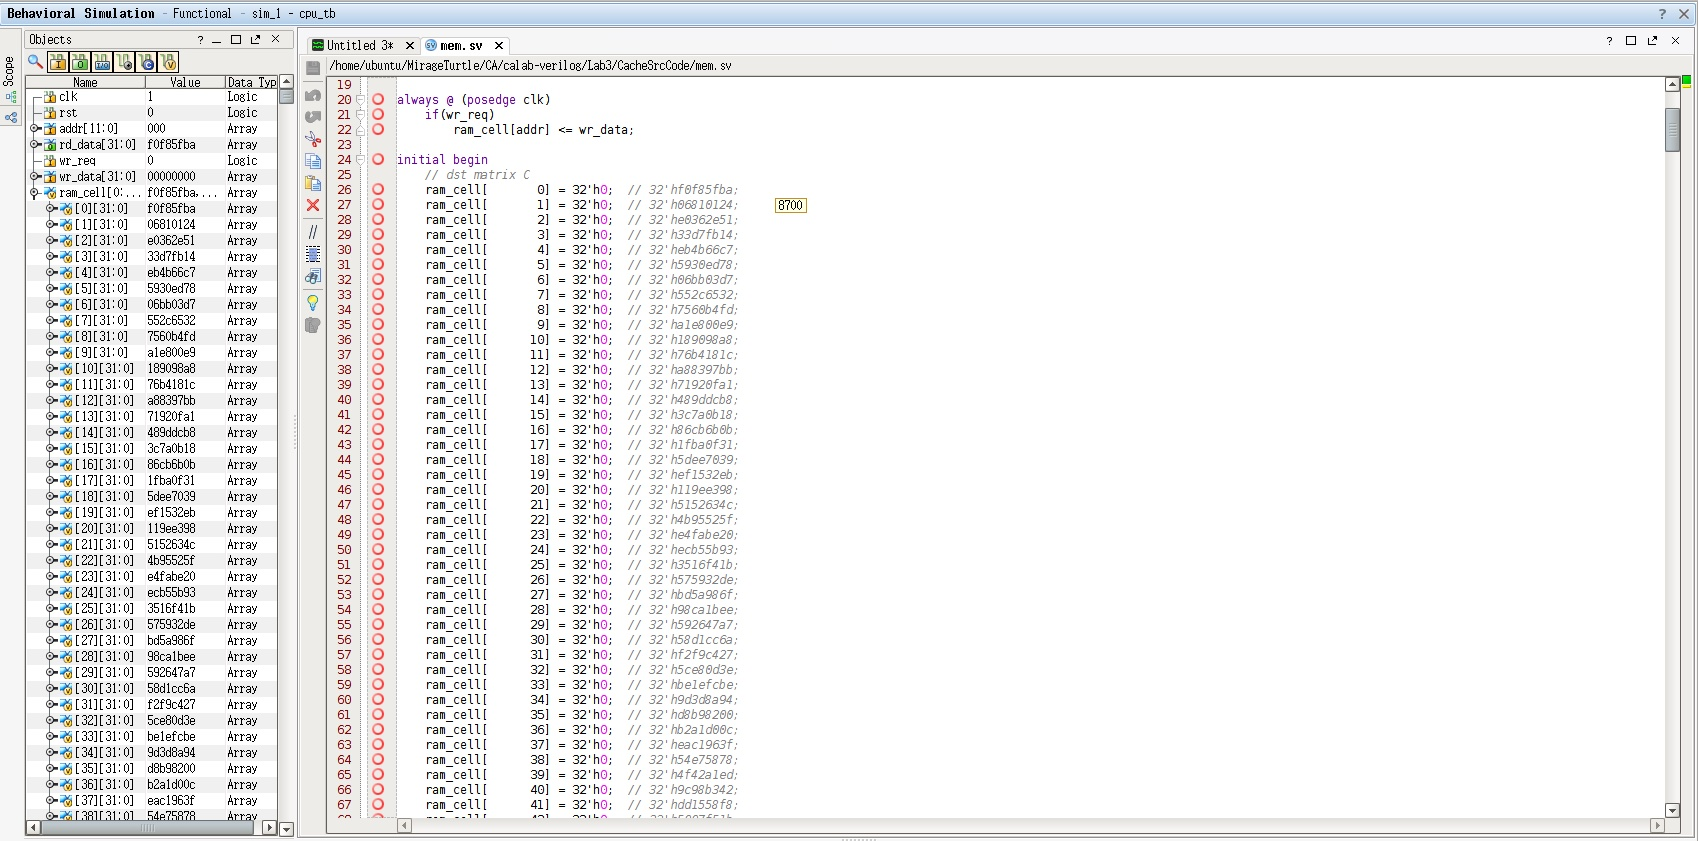
\includegraphics[width=0.4\textwidth]{./fig/stage2_fifo_matrix.jpg}
            }
        \end{figure}
        \item LRU策略
        \begin{figure}[H]
            \centering
            \subfigure[快排]{
                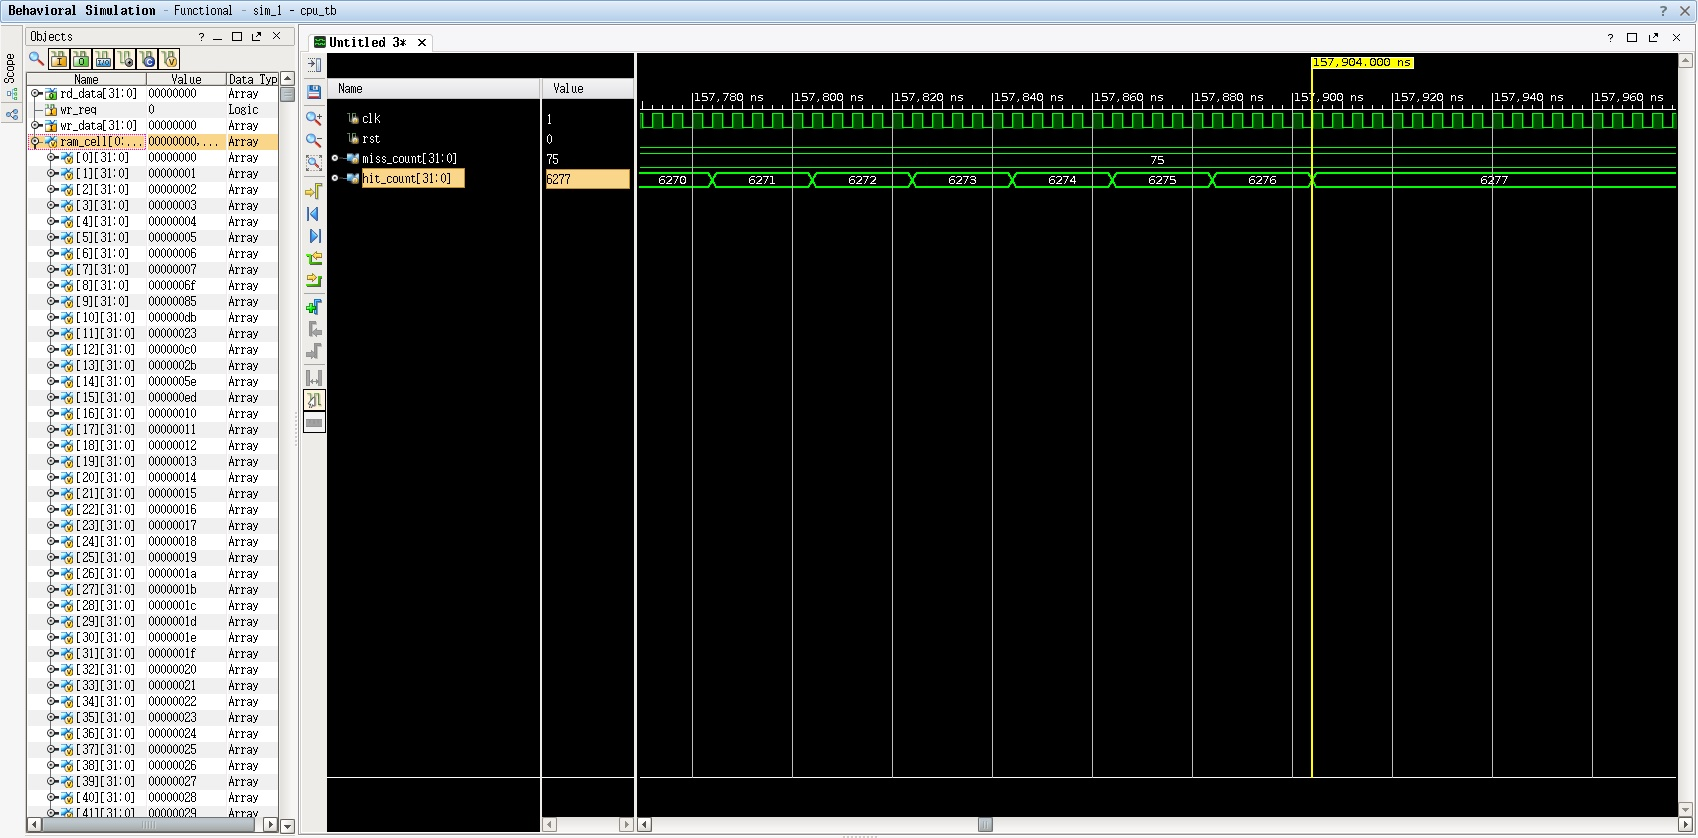
\includegraphics[width=0.4\textwidth]{./fig/stage2_lru_qsort.jpg}
            }
            \subfigure[矩阵乘法]{
                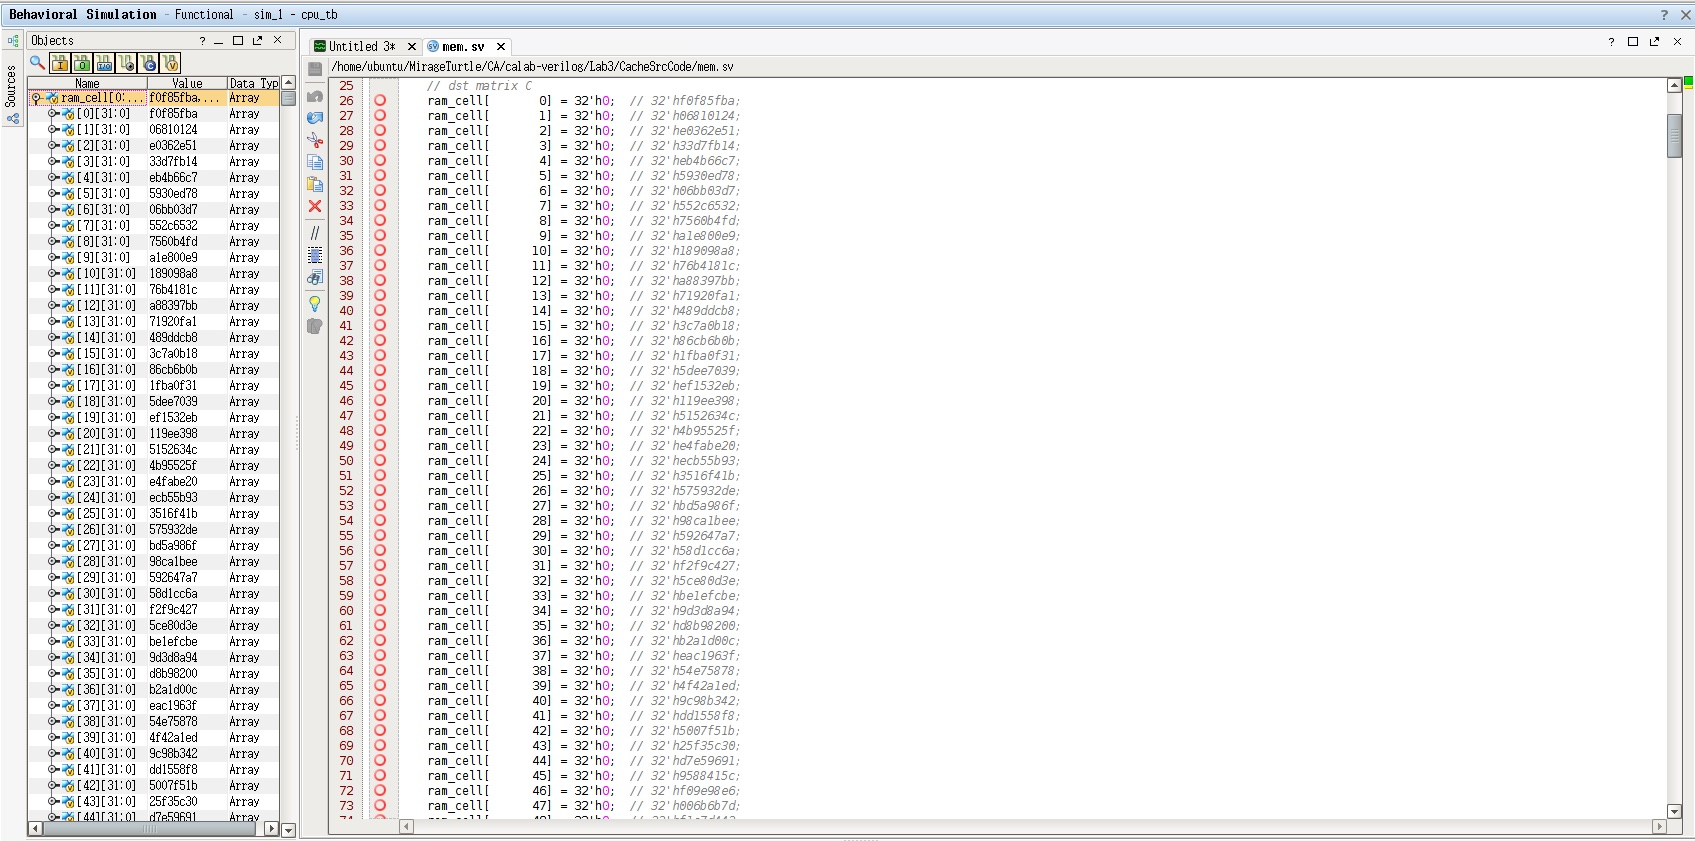
\includegraphics[width=0.4\textwidth]{./fig/stage2_lru_matrix.jpg}
            }
        \end{figure}
    \end{enumerate}
    可以看出矩阵乘法的结果与预期结果一致,快排结果大部分都是有序的,
    其中少部分乱序是由于cache的存在,部分结果没有写回内存中。
    \subsection{性能分析}
    \begin{table}[H]
        \centering
        \caption{FIFO策略下进行快排序}
        \begin{tabular}{cccccccc}
            \hline
            {\jetbrains LINE\_ADDR\_LEN} & {\jetbrains SET\_ADDR\_LEN} & {\jetbrains TAG\_ADDR\_LEN} & {\jetbrains WAY\_CNT} & Time(ns) & miss & hit & miss\_rate \\
            \hline
            3 & 3 & 6 & 4 & 150912 & 59 & 6293 & 0.93\% \\
            \hline
            3 & 3 & 6 & 2 & 188224 & 148 & 6204 & 2.33\% \\
            3 & 3 & 6 & 3 & 169760 & 102 & 6250 & 1.61\% \\
            \hline
            2 & 3 & 7 & 4 & 224440 & 256 & 6096 & 4.03\% \\
            4 & 3 & 5 & 4 & 136872 & 20 & 6332 & 0.31\% \\
            \hline
            3 & 2 & 7 & 4 & 184188 & 138 & 6216 & 2.17\% \\
            3 & 4 & 5 & 4 & 140976 & 39 & 6313 & 0.61\% \\
            \hline
        \end{tabular}
    \end{table}
    \begin{table}[H]
        \centering
        \caption{LRU策略下进行快排}
        \begin{tabular}{cccccccc}
            \hline
            {\jetbrains LINE\_ADDR\_LEN} & {\jetbrains SET\_ADDR\_LEN} & {\jetbrains TAG\_ADDR\_LEN} & {\jetbrains WAY\_CNT} & Time(ns) & miss & hit & miss\_rate \\
            \hline
            3 & 3 & 6 & 4 & 157904 & 75 & 6277 & 1.18\% \\
            \hline
            3 & 3 & 6 & 2 & 186328 & 144 & 6208 & 2.27\% \\
            3 & 3 & 6 & 3 & 167444 & 98 & 6254 & 1.54\% \\
            \hline
            2 & 3 & 7 & 4 & 227236 & 266 & 6086 & 4.18\% \\
            4 & 3 & 5 & 4 & 137720 & 22 & 6330 & 0.35\% \\
            \hline
            3 & 2 & 7 & 4 & 185260 & 161 & 6191 & 2.53\% \\
            3 & 4 & 5 & 4 & 141400 & 40 & 6314 & 0.63\% \\
            \hline
        \end{tabular}
    \end{table}
    \begin{table}[H]
        \centering
        \caption{FIFO策略下进行矩阵乘法}
        \begin{tabular}{cccccccc}
            \hline
            {\jetbrains LINE\_ADDR\_LEN} & {\jetbrains SET\_ADDR\_LEN} & {\jetbrains TAG\_ADDR\_LEN} & {\jetbrains WAY\_CNT} & Time(ns) & miss & hit & miss\_rate \\
            \hline
            3 & 3 & 6 & 4 & 150912 & 1739 & 8900 & 16.35\% \\
            \hline
            3 & 3 & 6 & 2 & 1363116 & 4864 & 5775 & 45.72\% \\
            3 & 3 & 6 & 3 & 1321644 & 4672 & 5967 & 43.91\% \\
            \hline
            2 & 3 & 7 & 4 & 1340684 & 4760 & 5881 & 44.73\% \\
            4 & 3 & 5 & 4 & 276516 & 72 & 10567 & 0.68\% \\
            \hline
            3 & 2 & 7 & 4 & 1349292 & 4800 & 5839 & 45.12\% \\
            3 & 4 & 5 & 4 & 293732 & 144 & 10495 & 1.35\% \\
            \hline
        \end{tabular}
    \end{table}
    \begin{table}[H]
        \centering
        \caption{LRU策略下进行矩阵乘法}
        \begin{tabular}{cccccccc}
            \hline
            {\jetbrains LINE\_ADDR\_LEN} & {\jetbrains SET\_ADDR\_LEN} & {\jetbrains TAG\_ADDR\_LEN} & {\jetbrains WAY\_CNT} & Time(ns) & miss & hit & miss\_rate \\
            \hline
            3 & 3 & 6 & 4 & 723800 & 1935 & 8704 & 18.19\% \\
            \hline
            3 & 3 & 6 & 2 & 1345188 & 4781 & 5858 & 44.94\% \\
            3 & 3 & 6 & 3 & 1191188 & 4089 & 6550 & 38.43\% \\
            \hline
            2 & 3 & 7 & 4 & 1299804 & 4590 & 6049 & 43.14\% \\
            4 & 3 & 5 & 4 & 295660 & 150 & 10489 & 1.41\% \\
            \hline
            3 & 2 & 7 & 4 & 1260868 & 4407 & 6232 & 41.42\% \\
            3 & 4 & 5 & 4 & 307956 & 205 & 10434 & 1.93\% \\
            \hline
        \end{tabular}
    \end{table}
    通过以上数据分析对比,可以得到以下结论:
    \begin{itemize}
        \item 随着{\jetbrains LINE\_ADDR\_LEN}、{\jetbrains SET\_ADDR\_LEN}、{\jetbrains WAY\_CNT}的增大,
        丢失率逐渐降低,即当增大cache容量时,cache存储数据量增加,命中率提高。
        \item 对于快排问题,LRU的效果与FIFO相差无几,且各有胜负,
        对于矩阵乘法问题,LRU效果略好于FIFO,但效果也不显著。
        \item 对于快排问题,计算量较小,cache容量增大产生的命中率提高并不明显(相较之下),
        但对于矩阵乘法问题,增大cache容量,能看到很明显的命中率提高,在某些情况下可能引起数量级上的改变。
    \end{itemize}

    \subsection{资源分析}
    在cache参数为{\jetbrains LINE\_ADDR\_LEN\ =\ 3\ SET\_ADDR\_LEN\ =\ 3\ TAG\_ADDR\_LEN\ =\ 6\ WAY\_CNT\ =\ 4},
    采用FIFO策略时,资源占用如下:
    \begin{figure}[H]
        \centering
        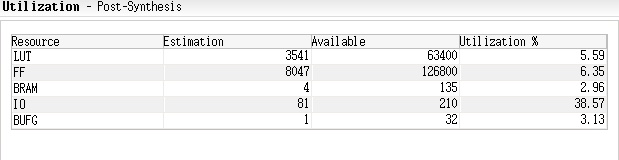
\includegraphics[width=0.8\textwidth]{./fig/utilization.jpg}
    \end{figure}
    由于篇幅原因,以下数据用表格形式展示。
    \begin{table}[H]
        \centering
        \caption{FIFO策略下的资源数量}
        \begin{tabular}{cccccc}
            \hline
            {\jetbrains LINE\_ADDR\_LEN} & {\jetbrains SET\_ADDR\_LEN} & {\jetbrains TAG\_ADDR\_LEN} & {\jetbrains WAY\_CNT} & {\jetbrains LUT} & {\jetbrains FF} \\
            \hline
            3 & 3 & 6 & 4 & 4270 & 10415 \\
            \hline
            3 & 3 & 6 & 2 & 2152 & 5678 \\
            3 & 3 & 6 & 3 & 3541 & 8047 \\
            \hline
            2 & 3 & 7 & 4 & 2738 & 5970 \\
            4 & 3 & 5 & 4 & 7741 & 19340 \\
            \hline
            3 & 2 & 7 & 4 & 2629 & 5695 \\
            3 & 4 & 5 & 4 & 7477 & 19823 \\
            \hline
        \end{tabular}
    \end{table}
    \begin{table}[H]
        \centering
        \caption{LRU策略下的资源数量}
        \begin{tabular}{cccccc}
            \hline
            {\jetbrains LINE\_ADDR\_LEN} & {\jetbrains SET\_ADDR\_LEN} & {\jetbrains TAG\_ADDR\_LEN} & {\jetbrains WAY\_CNT} & {\jetbrains LUT} & {\jetbrains FF} \\
            \hline
            3 & 3 & 6 & 4 & 4339 & 10417 \\
            \hline
            3 & 3 & 6 & 2 & 2458 & 5680 \\
            3 & 3 & 6 & 3 & 3598 & 8042 \\
            \hline
            2 & 3 & 7 & 4 & 2809 & 5972 \\
            4 & 3 & 5 & 4 & 7795 & 19342 \\
            \hline
            3 & 2 & 7 & 4 & 2696 & 5697 \\
            3 & 4 & 5 & 4 & 7615 & 19825 \\
            \hline
        \end{tabular}
    \end{table}
    从以上数据可以看出:
    \begin{itemize}
        \item 可以看出,cache容量的增加,会导致电路资源消耗更多,并且这种增长很快。
        \item 对照两种策略可以看出,FIFO和LRU的资源消耗并没有明显差异,
        原因可能是因为我FIFO和LRU采用了几乎相同的设计,
        区别较大的可能是FIFO在命中时不更新(都加1不影响相对大小),LRU在命中时更新。
    \end{itemize}
    \section{实验总结}
    \begin{enumerate}
        \item 通过本次Cache相关实验,我对cache有了更加清晰的认识,包括分类、工作原理、性能相关等等。
        \item 了解了Vivado的综合功能,也利用该功能进行了综合分析,也更加熟悉Verilog的编程。
        \item 同时也增加了一些cache设计、Vivado设计相关的经验。
    \end{enumerate}
\end{document}